% DPF 09 talk on strangeness in nucleon

\documentclass[10pt]{beamer}
\usefonttheme{professionalfonts} % using non standard fonts for beamer
\usefonttheme{serif} % default family is serif
\usepackage{amsmath}
\usepackage{mathtools}
\usepackage{mwe}
%\documentclass[12pt]{beamerthemeSam.sty}
\usepackage{epsf}
%\usepackage{pstricks}
%\usepackage[orientation=portrait,size=A4]{beamerposter}
\geometry{paperwidth=160mm,paperheight=120mm}
%DT favorite definitions
\def\LL{\left\langle}	% left angle bracket
\def\RR{\right\rangle}	% right angle bracket
\def\LP{\left(}		% left parenthesis
\def\RP{\right)}	% right parenthesis
\def\LB{\left\{}	% left curly bracket
\def\RB{\right\}}	% right curly bracket
\def\PAR#1#2{ {{\partial #1}\over{\partial #2}} }
\def\PARTWO#1#2{ {{\partial^2 #1}\over{\partial #2}^2} }
\def\PARTWOMIX#1#2#3{ {{\partial^2 #1}\over{\partial #2 \partial #3}} }

\def\rightpartial{{\overrightarrow\partial}}
\def\leftpartial{{\overleftarrow\partial}}
\def\diffpartial{\buildrel\leftrightarrow\over\partial}

\def\BI{\begin{itemize}}
\def\EI{\end{itemize}}
\def\BE{\begin{displaymath}}
\def\EE{\end{displaymath}}
\def\BEA{\begin{eqnarray*}}
\def\EEA{\end{eqnarray*}}
\def\BNEA{\begin{eqnarray}}
\def\ENEA{\end{eqnarray}}
\def\EL{\nonumber\\}


\newcommand{\map}[1]{\frame{\frametitle{\textbf{Course map}}
\centerline{\includegraphics[height=0.86\paperheight]{../../map/#1.png}}}}
\newcommand{\wmap}[1]{\frame{\frametitle{\textbf{Course map}}
\centerline{\includegraphics[width=0.96\paperwidth]{../../map/#1.png}}}}

\newcommand{\etal}{{\it et al.}}
\newcommand{\gbeta}{6/g^2}
\newcommand{\la}[1]{\label{#1}}
\newcommand{\ie}{{\em i.e.\ }}
\newcommand{\eg}{{\em e.\,g.\ }}
\newcommand{\cf}{cf.\ }
\newcommand{\etc}{etc.\ }
\newcommand{\atantwo}{{\rm atan2}}
\newcommand{\Tr}{{\rm Tr}}
\newcommand{\dt}{\Delta t}
\newcommand{\op}{{\cal O}}
\newcommand{\msbar}{{\overline{\rm MS}}}
\def\chpt{\raise0.4ex\hbox{$\chi$}PT}
\def\schpt{S\raise0.4ex\hbox{$\chi$}PT}
\def\MeV{{\rm Me\!V}}
\def\GeV{{\rm Ge\!V}}

%AB: my color definitions
%\definecolor{mygarnet}{rgb}{0.445,0.184,0.215}
%\definecolor{mygold}{rgb}{0.848,0.848,0.098}
%\definecolor{myg2g}{rgb}{0.647,0.316,0.157}
\definecolor{abtitlecolor}{rgb}{0.0,0.255,0.494}
\definecolor{absecondarycolor}{rgb}{0.0,0.416,0.804}
\definecolor{abprimarycolor}{rgb}{1.0,0.686,0.0}
\definecolor{Red}           {cmyk}{0,1,1,0}
\definecolor{Grey}           {cmyk}{.7,.7,.7,0}
\definecolor{Lg}           {cmyk}{.4,.4,.4,0}
\definecolor{Blue}          {cmyk}{1,1,0,0}
\definecolor{Green}         {cmyk}{1,0,1,0}
\definecolor{Brown}         {cmyk}{0,0.81,1,0.60}
\definecolor{Black}         {cmyk}{0,0,0,1}

\usetheme{Madrid}
\newcommand{\vcenteredinclude}[1]{\begingroup
  \setbox0=\hbox{\includegraphics[width=3in]{#1}}%
\parbox{\wd0}{\box0}\endgroup}

%AB: redefinition of beamer colors
%\setbeamercolor{palette tertiary}{fg=white,bg=mygarnet}
%\setbeamercolor{palette secondary}{fg=white,bg=myg2g}
%\setbeamercolor{palette primary}{fg=black,bg=mygold}
\setbeamercolor{title}{fg=abtitlecolor}
\setbeamercolor{frametitle}{fg=abtitlecolor}
\setbeamercolor{palette tertiary}{fg=white,bg=abtitlecolor}
\setbeamercolor{palette secondary}{fg=white,bg=absecondarycolor}
\setbeamercolor{palette primary}{fg=black,bg=abprimarycolor}
\setbeamercolor{structure}{fg=abtitlecolor}

\setbeamerfont{section in toc}{series=\bfseries}

%AB: remove navigation icons
\beamertemplatenavigationsymbolsempty
\title{
  \textbf {Resonant modes in interesting shapes}\\
%\centerline{}
%\centering
%\vspace{-0.0in}
%\includegraphics[width=0.3\textwidth]{propvalues_0093.pdf}
%\vspace{-0.3in}\\
%\label{intrograph}
}

\author[W. Freeman] {Physics 211\\Syracuse University, Physics 211 Spring 2015\\Walter Freeman}

\date{\today}

\begin{document}

\frame{\titlepage}

\frame{\frametitle{\textbf{Announcements}}
  \Large
\BI
\item{Homework 9 due next Wednesday}
\item{Practice exam posted; 8 questions on it can be submitted for extra credit (also Wednesday)}
\item{Daily practice questions and discussion on the Facebook group (a new question will go up when someone answers the existing one!)}
\EI
}

\frame{\frametitle{\textbf{Announcements}}
  \Large
\BI
\item{Academic Scheduling still hasn't gotten back to me about a review schedule}
\item{I've asked for large blocks of time this Friday, and next Tuesday, Wednesday, and Thursday}
\item{I will let you all know what rooms I can get and when as soon as I know}
\item{Regardless, I will be available for extra help in one form or another a great deal:}
  \BI
\item{Check the Clinic}
\item{Check my office (313)}
\item{Email or Facebook message me to set up an appointment}
  \EI
  \EI
}



\frame{\frametitle{\textbf{Standing waves, from before}}
  \Large
  \vcenteredinclude{mode1-crop.pdf} Fundamental: $f_1 = \frac{c}{2L}$\\
 \bigskip 
  \vcenteredinclude{mode2-crop.pdf} 2nd harmonic: $f_2 = 2 f_1 $\\
 \bigskip 
  \vcenteredinclude{mode3-crop.pdf} 3rd harmonic: $f_3 = 3 f_1$ \\
  
 \bigskip 
  \vcenteredinclude{mode4-crop.pdf} 4th harmonic: $f_4 = 4 f_1$ \\
  
 \bigskip 

}



\frame{\frametitle{\textbf{Musical instruments: fun with spectroscopy}}
  \large
  \BI
\item{In general, when you excite a string or air column, you produce a combination of many standing wave modes}
\item{The unique sound of each instrument comes mostly from the relative strengths of them}
  \BI
\item{``Dark'' or ``pure'' sound: weak higher harmonics}
\item{``Bright'' or ``brassy'' sound: strong higher harmonics}
  \EI
\item{All of these pitched instruments have evenly-spaced frequencies}
\item{This is necessary for something to sound like a musical note}
\item{Strings and uniform tubes do this naturally}
\item{If we want to make an instrument out of another shape, we have to eliminate ``non-harmonic'' frequencies}
  \EI
}

\frame{\frametitle{\textbf{A simple example: the xylophone and its cousins}}
\Large
Instrument made from wooden bars: small ones are high notes, big ones are low notes
\bigskip
\centerline{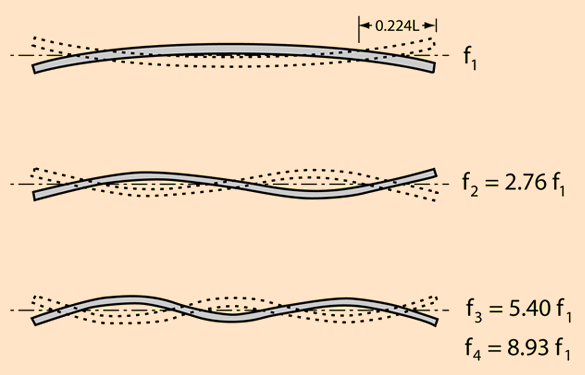
\includegraphics[width=0.5\textwidth]{bar-modes.png}}
\bigskip
We have a problem: the frequencies of the normal modes are {\it not harmonic!}; they don't form ratios of 1, 2, 3, 4...
\normalsize
\BI
\item{If these are allowed to vibrate, the instrument won't sound like a single musical pitch}
\pause
\item{Solution: support the bar at the nodes of the first mode}
\item{This allows that mode to vibrate, but damps out the others that don't have nodes there}
\item{The peculiar sound of the marimba comes from the rapid decay of these non-harmonic modes}
  \EI
}

\frame{\frametitle{\textbf{Normal modes for other shapes}}
  \large
\BI
\item{In general, other shapes have a huge diversity of (very interesting) vibrational modes!}
\item{A few examples...}
  \pause
\item{Simulations:}
  \BI
\item{Square membrane: acts like a string in two dimensions, but with {\it two} numbers needed (number of antinodes in x and y)}
\item{Circular membrane: like a drumhead, along with its properties}
  \EI
\item{Real examples}
  \BI
\item{Chladni plates}
\item{Other fancy toys...}
  \EI
  \EI
}

\frame{\frametitle{\textbf{Far more than just acoustics!}}
  \large
  \BI
\item{These ideas of resonance and normal modes apply to {\it anything} that can oscillate!}
\item{Key ideas:}
  \BI
\item{An object can vibrate in particular ways determined by its structure}
\item{Each of those {\bf normal modes} has a particular frequency}
\item{It absorbs energy very readily at those frequencies}
  \EI
\item{Electric circuits: antennas (standing waves in a wire!), and the equivalent of masses on strings}
\item{Mechanical designs of all sorts of things}
  \pause
\item{Architecture: {\color{Red} \bf resonance is very bad...}}
  \pause
\item{Lots of work goes into ensuring that there are no strong resonances where there shouldn't be any...}
  \EI
}
  \frame{\frametitle{\textbf{Quantum mechanics and the connection to chemistry}}
    \centerline{\Large\color{Red} A key idea in quantum mechanics: matter is made of waves, too}
    \large
    \BI
  \item{Are there normal modes for atoms, too?}
    \pause
  \item{You bet! These standing wave patterns (for matter waves) are the orbitals you study in chemistry!}
    \EI
  \bigskip
  \bigskip
  \centerline{  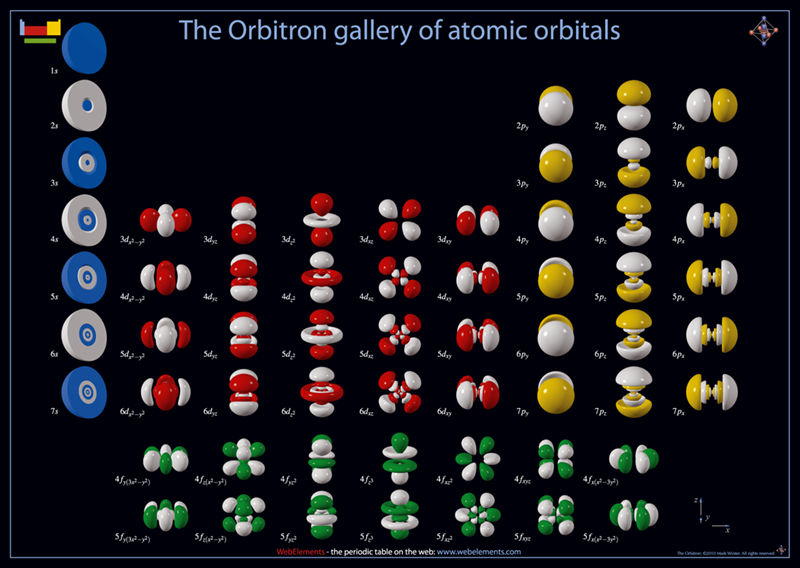
\includegraphics[width=0.55\textwidth]{orbitals.jpg}}
  \bigskip
  \bigskip
  \centerline {\normalsize  Great advances in quantum mechanics were made by people thinking about violin strings!}

  
}

\frame{\frametitle{\textbf{Resonance appears everywhere...}}
  \large
  \BI
\item{Studying the resonant modes of molecules can tell us a great deal!}
\item{Every molecule has certain resonant frequencies}
  \BI
\item{Think of the mechanics of molecular bonds flexing...}
\item{This involves the combination of the laws of motion you learned here, plus quantum mechanics}
  \EI
\item{``Light'', too, is a wave}
\item{We can study strings by looking at how they couple to sound waves...}
\item{... physicists and chemists study atoms and molecules by looking at how they couple to light waves!}
\item{Going even smaller, particle physicists do the same thing: we even mix up the words!}
\item{You might even say: all of science appears in the concert hall!}
  \EI
}

\frame{\frametitle{\textbf{I leave you with two quotes...}}
\pause
``A poet once said, 'The whole universe is in a glass of wine.'...  [I]f we look at a glass of wine closely enough we see the entire universe. 
There are the things of physics: the twisting liquid which evaporates depending on the wind and weather, the reflection in the glass; and our imagination adds atoms. 
The glass is a distillation of the earth's rocks, and in its composition we see the secrets of the universe's age, and the evolution of stars. 
What strange array of chemicals are in the wine? 
How did they come to be? 
There are the ferments, the enzymes, the substrates, and the products. 
There in wine is found the great generalization; all life is fermentation. 
Nobody can discover the chemistry of wine without discovering, as did Louis Pasteur, the cause of much disease. 
How vivid is the claret, pressing its existence into the consciousness that watches it! 
If our small minds, for some convenience, divide this glass of wine, this universe, into parts -- physics, biology, geology, astronomy, psychology, 
and so on -- remember that nature does not know it! So let us put it all back together, not forgetting ultimately what it is for. Let it give us one more final pleasure; drink it and forget it all!''

\bigskip
\bigskip

\pause

``Poets say science takes away from the beauty of the stars — mere globs of gas atoms. Nothing is "mere". I too can see the stars on a desert night, and feel them. But do I see less or more? The vastness of the heavens stretches my imagination — stuck on this carousel my little eye can catch one-million-year-old light. A vast pattern — of which I am a part... What is the pattern, or the meaning, or the why? It does not do harm to the mystery to know a little about it. For far more marvelous is the truth than any artists of the past imagined!''

--Richard Feynman, from {\em Lectures on Physics}
}
\end{document}
